\chapter{Part1: Basic terminologies and notions}

\subsection{System Response}
In automatic control, the response of a system to an external input can be decomposed into two components: the \textit{zero-input response} and the \textit{zero-state response}. These two components describe how the system behaves due to its initial conditions and external inputs, respectively.

\subsubsection{Zero-Input Response}
The \textbf{zero-input response} refers to the system's response solely due to the initial conditions of the system, assuming there is no external input applied. Mathematically, for a linear time-invariant (LTI) system, the zero-input response is governed by the system's natural dynamics. If the state-space representation of the system is:

\[
\dot{x}(t) = Ax(t) + Bu(t),
\]
where \(x(t)\) is the state vector, \(A\) is the system matrix, and \(u(t)\) is the input, the zero-input response is the solution of the homogeneous system:
\[
\dot{x}(t) = Ax(t), \quad u(t) = 0.
\]
The general solution for the zero-input response is:
\[
x_{zi}(t) = e^{At}x(0),
\]
where \(x(0)\) represents the initial state of the system.

\subsubsection{Zero-State Response}
The \textbf{zero-state response}, on the other hand, describes the system's response due only to the external input, assuming the system starts with zero initial conditions. For the same LTI system, the zero-state response is given by:
\[
x_{zs}(t) = \int_0^t e^{A(t-\tau)}Bu(\tau) \, d\tau,
\]
where \(u(t)\) is the input applied to the system.

The total response of the system is the sum of the zero-input and zero-state responses:
\[
x(t) = x_{zi}(t) + x_{zs}(t).
\]

\subsubsection{System Stability}

System stability is a fundamental concept in control theory and can be analyzed in terms of \textit{internal stability} and \textit{BIBO (Bounded-Input, Bounded-Output) stability}.

\subsubsection{Internal Stability}
A system is said to have \textbf{internal stability} if its natural response (the zero-input response) does not grow unbounded over time. This implies that, regardless of the initial conditions, the state of the system remains bounded as time progresses. For a linear system described by \( \dot{x}(t) = A x(t) \), internal stability can be analyzed by examining the eigenvalues of the matrix \(A\):

\begin{itemize}
    \item The system is \textit{asymptotically stable} if all eigenvalues of \(A\) have negative real parts. In this case, \( x(t) \to 0 \) as \( t \to \infty \), implying that the system's natural response decays over time.
    \item The system is \textit{marginally stable} if all eigenvalues of \(A\) have non-positive real parts, and any eigenvalues with zero real parts are simple (i.e., have a geometric multiplicity of 1). In this case, the system does not grow unbounded, but it may not decay to zero either.
    \item The system is \textit{unstable} if any eigenvalue of \(A\) has a positive real part. This results in an unbounded natural response.
\end{itemize}


\subsubsection{BIBO Stability}
A system is \textbf{BIBO stable} if, for every bounded input, the output remains bounded. In other words, if \( u(t) \) is bounded, meaning there exists some constant \( M \) such that \( |u(t)| \leq M \) for all \( t \), then the system output \( y(t) \) must also remain bounded.

For a linear system, BIBO stability can be determined by examining the system's transfer function \( H(s) \). The system is BIBO stable if and only if all poles of \( H(s) \) have negative real parts, i.e., they lie in the left half of the complex plane.

\subsubsection{Conclusion}
Understanding the zero-input and zero-state responses allows us to analyze how a system reacts to different conditions, while stability analysis ensures that the system behaves in a controlled manner over time. Both internal and BIBO stability are essential for ensuring that the system does not exhibit unbounded behavior in response to initial conditions or external inputs.


\subsubsection{Internal and BIBO stability of a system}
If an isolated system is available, two kind of stability needs to be studied:
\begin{itemize}
\item\textbf{internal stability}:as to zero-input response of the system
\item\textbf{BIBO stability}:as to the zero-state response of the system
\end{itemize}

\subsubsection{Internal Stability of the system}
Through the mathematical definition of stability, per se, stability of the system cannot be discussed in practice. That is, it is not possible to check the boundedness of the output for all the inputs possible. \textbf{In practice}, the knowledge that the response of a system is a linear combination of its \textit{\textbf{natural modes}} is exploited. Therefore:
\begin{itemize}
    \item a system is \textbf{internally stable} \(\iff \) all the natural modes of the system are stable.
    \item a system is \textbf{asymptotically stabl} \(\iff \) all the natural modes of the system are asymptotically stable.
    \item a system is \textbf{unstable} \(\iff \) there exist one unstable natural mode.
\end{itemize}
As you remember, system mode are exponential functions of eigenvalues of the system.

In analysing the eigenvalues of small matrices, the following propositions come in handy:
\begin{itemize}
    \item Descarte's rule of signs.
    \item Calculating Eigenvalues of a block-diagram matrices.
\end{itemize}

\begin{factbox}[Pay Attention]
Unlike the non-linear context where the stability is a characteristic of equiliblia, in linear context, stability is a property of the system.
\end{factbox}

\begin{QandAbox}[Question: HOW TO DEAL WITH THE OVERFLOW OF REAL INTEGRATORS? A REAL INTEGRATOR CANNOT ASSUME VERY LARGE VALUES.]
This problem is discussed under the title of anti wind-up controll.
\end{QandAbox}


\subsubsection{BIBO stability of the system}
Here, again the definition of BIBO stability cannot be used to guarantee the stability of the system. However, it can be used to prove the otherwise. In other words, whether a bounded input can be find that make the system unstable. This input usually increases the geometrical multiplicity of eigenvalues, or poles, with zero real part, leading to unbounded input as a consequence of the act of integration for integrators or resounance of systems resembling second-order systems.
\begin{example}[Example of unstable BIBO stable systems]
Consider the following operational amplifier; all the elements are considered to be idea.
\begin{figure}[H]
    \centering
    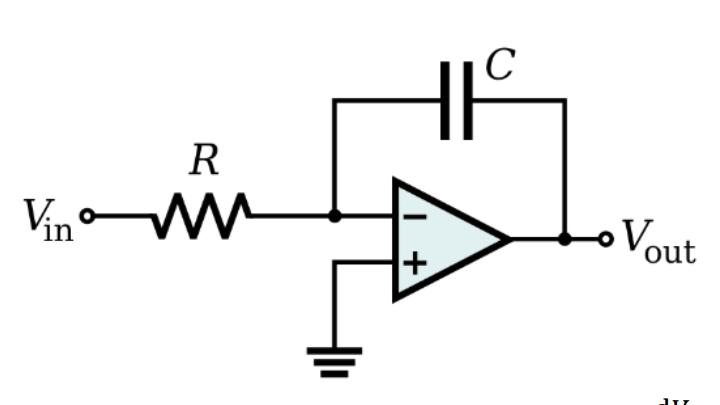
\includegraphics[width=0.5\textwidth]{integrator.png}
    \caption{An operational amplifier in an integrator setting}
    \label{fig:integrator}
\end{figure}
The input/output, or Transfer function, of the system can be written as follows:
\[
\frac{V_o}{V_i} = -\frac{z_2}{z_1} = \frac{-\frac{1}{Cs}}{R} = -\frac{1}{CRs}
\]
In this example, the capacitor \(C\) acts as an integrator, as it can be seen mathematically as \(H(s) = \frac{1}{s}\). In this case, if a unit step input is applied to the system, \(V_i(s) = \frac{1}{s}\), the output of the system is unbounded. It can be understood as follows:
\[
\lim_{t \to \infty} \int_{0}^{t} V_i(\tau) \, d\tau = 
\lim_{t \to \infty} \int_{0}^{t} \mathcal{E}(\tau) \, d\tau =
\lim_{t \to \infty} F(t) - F(0) = \lim_{t \to \infty} t - 0 = \infty
\]
which mean the system is BIBO unstable.
\end{example}
\begin{example}
Another example of integrator is a water reservoir.

Now, consider the following circuit, which is a resaunator circuit:

\begin{figure}[H]
    \centering
    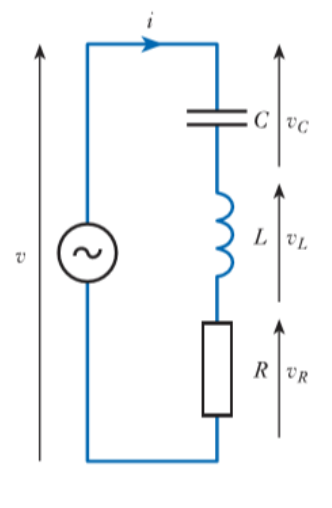
\includegraphics[width=0.25\textwidth]{resonator.png}
    \caption{a resonator circuit}
    \label{fig:resonator}
\end{figure}
The input-output relation of this circuit is as follows:
\[
I(s) = \frac{\frac{s}{L}}{s^2 + \frac{R}{L}s + \frac{1}{LC}} V(s)
\]
The natural frequency of this system is \(\omega = \frac{1}{\sqrt{LC}}\). If the value of the resistance \(R\) is zero in this system, by applying an input voltage with the aforementioned frequency, the current, theoretically, tends to infinity. 
\end{example}


In order for a system to be BIBO stable, the real part of all the poles of the system should be strictly smaller than zero.


\begin{QandAbox}[BIBO stable and Internally unstable]
Since there might be some cancellation between when shaping the transfer function of a system, \(H(s) = C(sI-A)^{-1}B + D)\), the poles of the system are a subset of the eigenvalues of the system matrix \(A\):\\

Poles(\(H(s)\)) \(\subseteq\) eig(\(A\)).\\

Hence, it can be concluded that if a system is asymptotically stable, then the system is also BIBO stable. However, the converse may not always be the case. Specifically, a system can be BIBO stable, but this does not guarantee that no zero-pole cancellation has occurred.\\

There may be cases where a system is \textbf{internally unstable} but \textbf{BIBO stable}. In such cases, one of the following two possibilities holds:

\end{QandAbox}
\begin{QandAbox}

\begin{itemize}
   \item The unstable mode of the system is \textbf{unreachable}, meaning that the input signal cannot stimulate that mode of the system.
   \item The unstable mode of the system is \textbf{unobservable}, meaning that while the input signal stimulates that mode, its effect does not appear in the output. This situation may lead to instability of the system itself.
\end{itemize}
\end{QandAbox}

The architecture of the control system discussed in this course is as follows:

\begin{figure}[H]
    \centering
    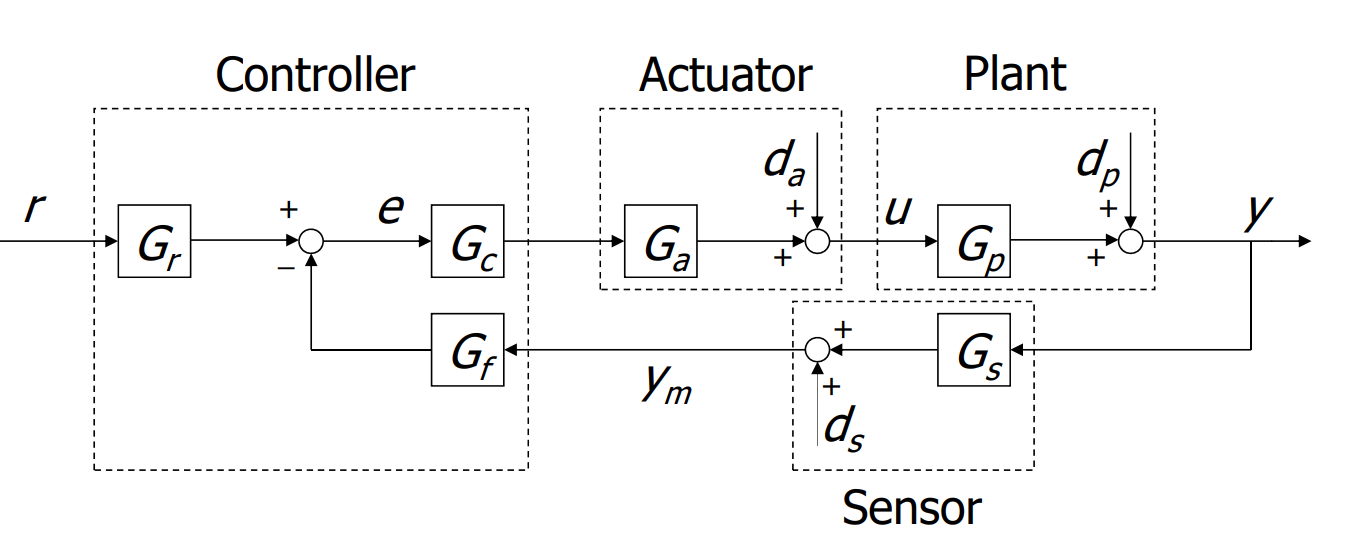
\includegraphics[width=0.75\textwidth]{control-architecture.png}
    \caption{The architecture of the control system discussed in this course}
    \label{fig:control-architecture}
\end{figure}
In the figure \ref{fig:control-architecture}, the symbols are as follows:
\begin{itemize}
    \item plant \(G_p\) with plant disturbance \(d_p\) 
    \item actuator \(G_a\) with actuator disturbance \(d_a\)
    \item sensor \(G_s\) with sensor noise \(d_s\)
    \item \textbf{cascade controller} \(G_c\)
    \item \textbf{feedback controller} \(G_f\), for 2 DoF or, if constant for dc-gain
    \item \textbf{prefilter} \(G_r\), also called reference generator
\end{itemize}

\textbf{Prefilter, or reference generator}, is not going to be discussed in this course. For instance, If an aircraft aims to land, the input of the system cannot be a step. The aircraft should follow a smooth path for landing. Therefore, prefilter does this job.

Let us consider the structure in the figure \ref{fig:our-control-system}. The multivariable transfer function \(M(s)\) from inputs signals \(r, d_u, \), and \(d_t\) to outputs signals \(e, u\), and \(y_m\) is given by:

\[
\begin{bmatrix}
e \\
u \\
y_m
\end{bmatrix}
=
\frac{1}{1 + PCF}
\begin{bmatrix}
1 & -PF & -F \\
C & 1 & -CF \\
PC & P & 1
\end{bmatrix}
\begin{bmatrix}
r \\
d_u \\
d_t
\end{bmatrix}
\]

\begin{figure}[H]
    \centering
    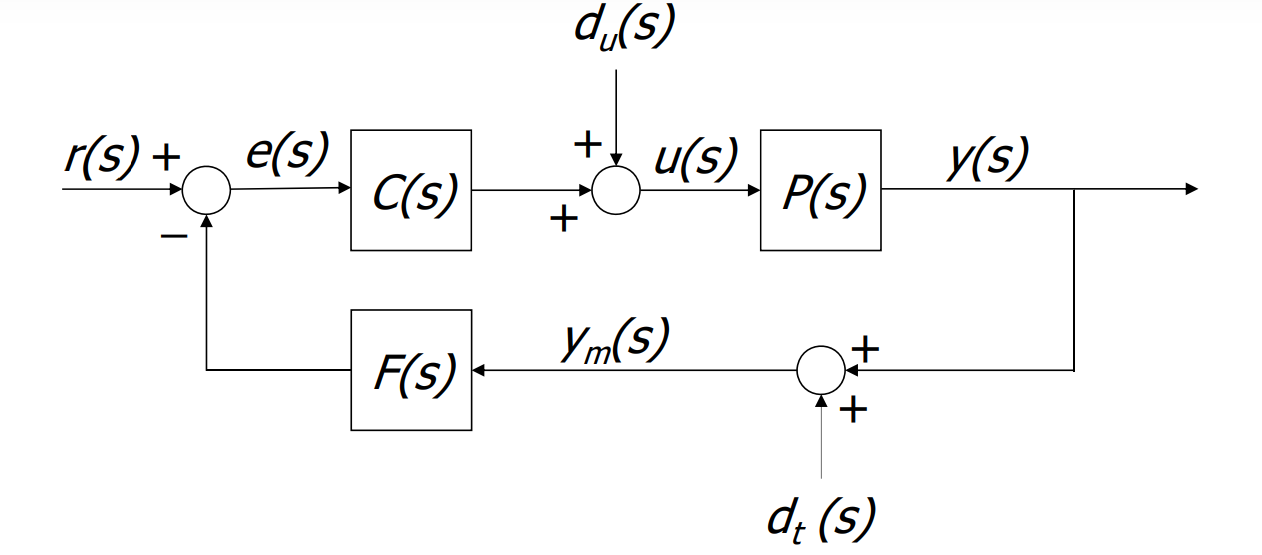
\includegraphics[width=0.75\textwidth]{our-control-system.png}
    \caption{The control architecture discussed for the following arguments}
    \label{fig:our-control-system}
\end{figure}

Based on this figure, we have the following definitions:
\begin{itemize}
    \item \textbf{loop-function} as\(L(s) = P(s)C(s)F(s)\)
    \item \textbf{sensitivity function} as \(S(s) =\left[1 + L(s)\right]^{-1}\)
    \item \textbf{complementary sensitivity function} as \(T(s) = 1- S(s)\)
\end{itemize}

\subsubsection{Well-posedness or closed-loop properness}
A feedback control system is said to be \textit{well-posed} or \textit{close-loop proper} if the closed-loop transfer function of every possible input-output pair of the system is proper.

The result of the \textit{well-posedness
}: The feedback control system is said to be well-posed if and only if:
\[
\lim \limits_{s \to \infty} \left\{1 + P(s)C(s)F(s)\right\} \neq 0
\]

\begin{factbox}[Physical interpretation of properness]
If the transfer fucntion of a physical system is not proper, in the time-domain, it implies that the state of the system at a given time instance depend on the future value of the input. This is in contradiction with causality, and therefore, physically unrealizable.

In the frequency domain, the final shape of the system's frequency response would be like that of a high-pass filter, meaning that the system would amplify high-frequency inputs, such as noise.
\end{factbox}

\subsubsection{Internal stability of feedback systems}
Let us assume that the plant \(P(s)\) to be controlled is \textit{\textbf{stabilizable}} by the input \(u\) - i.e. if all unstable modes are controllable - and \textit{\textbf{detactable}} through output \(y\) - i.e. if all unstable modes are observable. 

Having assumed that, the feedback system is said to be \textit{\textbf{internally stable}} if and only if the signals \(e, u\), and \(y_m\) are bounded for any possible choice of the bounded signals \(r, d_u\), and \(d_t\) - i.e if and only if all the transfer functions in \(M(s)\) are proper and BIBO stable.

\textbf{Results}:\\
The closed loop system considered here is stable if and only if the following considtions are met:
\begin{enumerate}
    \item all roots of the equation \(1 + L(s) = 0\) have real part strictly smaller than \(0\).
    \item there are no cancellations in \(\mathbb{Re}(s)\geq 0 \) when the product \(P(s)C(s)S(s)\) is formed.
\end{enumerate}

\textbf{Remarks}:
\begin{itemize}
    \item No proof is given.
    \item Consition (1) follows the fact that the poles of all the functions in \(M(s)\)) are roots of the equation \(1 + L(s) = 0\);
\end{itemize}

